\section{Tooling}\label{sec:tooling}

\subsection{ATM}\label{sec:descriptionaxini}
ATM is a web-based model-based testing application, developed in the Ruby on Rails framework. It is used to test the software of several big companies in the Netherlands since 2006. It is under continuous development by Axini.

The architecture is shown graphically in Figure~\ref{fig:axini_tool}. It has a similar structure to the on-the-fly model-based testing tool architecture in Figure~\ref{fig:model_based_testing_on_the_fly}.

\begin{figure}[h!]
  \begin{center}
    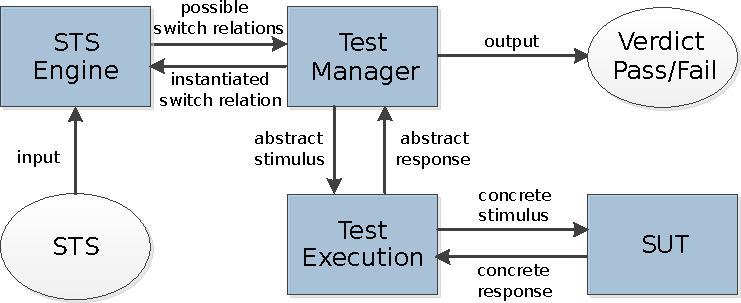
\includegraphics[width=0.75\textwidth]{axini_tool.pdf}
  \end{center}
  \caption{Architecture of ATM}
  \label{fig:axini_tool}
\end{figure}

The tool functions as follows: 
\begin{enumerate}
  \item An STS is given to an STS Engine, which keeps track of the current location and data values. It passes the possible switch relations from the current location to the Test Manager.
  \item The Test Manager chooses a switch relation and the data values based on a test strategy. The choice is represented by an instantiated switch relation and passed back to the STS Engine, which updates its current location and data values. The communication between these two components is done by method calls.
  \item The gate of the instantiated switch relation is given to the Test Execution component as an \textit{abstract stimulus}. The term abstract indicates that the instantiated switch relation is an abstract representation of some computation steps taken in the SUT. For instance, a transition with label 'connect?' is an abstract stimulus of the actual setup of a TCP connection between two distributed components of the SUT. 
  \item The translation of an abstract stimulus to a concrete stimulus is done by the Test Execution component. This component provides the stimulus to the SUT. When the SUT responds, the Test Execution component translates this response to an abstract response. For instance, the Test Execution component receives an HTTP response that the TCP connect was succesful. This is a concrete response, which the Test Execution component translates to an abstract response, such as a transition with label 'ok!'. The Test Manager is notified with this abstract response.
  \item The Test Manager translates the abstract response to an instantiated switch relation and updates the STS Engine. If this is possible according to the model, the Test Manager gives a pass verdict for this test. Otherwise, the result is a fail verdict.
\end{enumerate}

\subsection{GROOVE}\label{sec:descriptiongroove}
GROOVE is an open source, graph-based modelling tool in development at the University of Twente since 2004. \cite{Rensink2003a}\marginpar{read and summarize this paper}. It has been applied to several case studies, such as model transformations and security and leader election protocols~\cite{Ghamarian:GROOVE}.

The architecture of the GROOVE tool is shown graphically in Figure~\ref{fig:groove_tool}. A graph grammar is given as input to the Rule Applier component, which determines the possible rule transitions. An Exploration Strategy can be started or the user can explore the states manually using the GUI. These components request the possible rule transitions and respond with the chosen rule transition (based on the exploration strategy or the user input). The Exploration Strategy can do an exhaustive search, resulting in a GTS. The graph states and rule transitions in this GTS can then be inspected using the GUI.

\begin{figure}[h]
  \begin{center}
    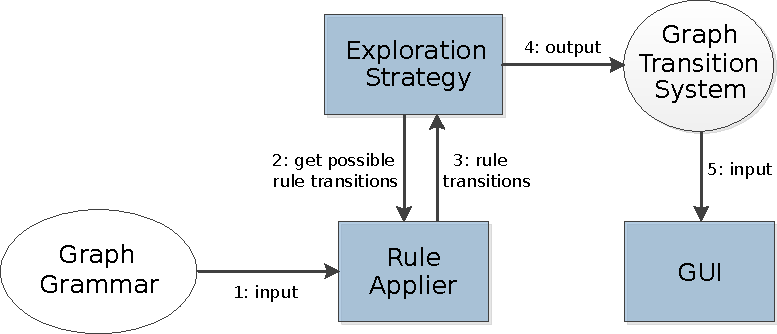
\includegraphics[width=0.75\textwidth]{groove_tool.pdf}
  \end{center}
  \caption{The GROOVE Tool}
  \label{fig:groove_tool}
\end{figure}

\subsection{GROOVE example}
The $\mathit{LHS}$, $\mathit{RHS}$ and $\mathit{NAC}$ of a rule in graph transformation tools, such as GROOVE, are often visualized together in one graph. The running example from Figure~\ref{fig:example_sts} is displayed as a graph grammar, as visualized in GROOVE, in Figure~\ref{fig:example_groove}. Figure~\ref{fig:example_groove_start} is the start graph of the system. The rules can be described as follows:
\begin{enumerate}
  \item~\ref{fig:example_groove_throw}: 'if a player has the turn and he has not thrown the die yet, he may do so.'
  \item~\ref{fig:example_groove_move}: 'if a player has the turn and he has thrown the die and this number is larger than zero, he may move one place and then it is as if he has thrown one less.'
  \item~\ref{fig:example_groove_next}: 'if a player has finished moving (number thrown is zero), the next player receives the turn.'
\end{enumerate}

The colors on the nodes and edges in the rules represent   they belong:
\begin{enumerate}
  \item normal line (black): This node or edge is part of both the $\mathit{LHS}$ and $\mathit{RHS}$. $\mathit{Map}$ contains the mapping of this node as part of the $\mathit{LHS}$ to itself as part of the $\mathit{RHS}$.
  \item dotted line (red): This node or edge is part of the $\mathit{NAC}$ only.
  \item thick line (green): This node or edge is part of the $\mathit{RHS}$ only.
  \item dashed line (blue): This node or edge is part of the $\mathit{LHS}$ only.
\end{enumerate}

The $turn$ flag on the \textbf{Player} node is a representation of a self-edge with label $turn$. The assignments on the \textbf{Die} node are representations of edges to integer nodes. The throws value assignment (:=) in the move rule is a shorthand for two edges: one edge in the $\mathit{LHS}$ with label $throws$ from the \textbf{Player} node to an integer node with value $i$ and another edge in the $\mathit{RHS}$ with label $throws$ from the \textbf{Player} node to an integer node with value $i-1$. In the next turn rule, the $turn$ edge exists in the $\mathit{LHS}$ as a self-edge of the left \textbf{Player} node and in the $\mathit{RHS}$ as a self-edge of the right \textbf{Player} node. In the same rule, the $throws$ edge from the left \textbf{Player} node to an integer node only exists in the $\mathit{LHS}$. The number '0' in the top left of the \textbf{int} node in the throw rule indicates that this integer is the first parameter on the rule transition when this rule is applied. 

\begin{figure}[h!]
  \begin{center}
    \subfloat[The start graph]{\label{fig:example_groove_start}% To use this figure in your LaTeX document
% import the package groove/resources/groove2tikz.sty
%
% Special colors
\begin{tikzpicture}[
% Special color styles
scale=\tikzscale]
\node[node] (n0)  at (2.250, -0.605) {\ml{\textbf{Die}\\rolls = 0}};
\node[node] (n10)  at (3.560, -2.025) {\ml{\textbf{Location}}};
\node[node] (n9)  at (0.930, -1.985) {\ml{\textbf{Location}}};
\node[node] (n8)  at (2.200, -2.545) {\ml{\textbf{Location}}};
\node[node] (n11)  at (0.990, -0.600) {\ml{\textbf{Player}\\\textit{turn}\\id = 1}};
\node[node] (n7)  at (2.180, -1.465) {\ml{\textbf{Location}}};
\node[node] (n12)  at (3.550, -0.615) {\ml{\textbf{Player}\\id = 2}};
\path[edge](n11.south -| 0.930, -1.985) -- node[lab]{at} (n9) ;
\path[edge] (n10)  -- node[lab]{next} (n8) ;
\path[edge] (n9)  -- node[lab]{next} (n7) ;
\path[edge] (n8)  -- node[lab]{next} (n9) ;
\path[edge] (n7)  -- node[lab]{next} (n10) ;
\path[edge](n12.south -| 3.560, -2.025) -- node[lab]{at} (n10) ;
\userdefinedmacro
\end{tikzpicture}
\renewcommand{\userdefinedmacro}{\relax}
}\quad
    \subfloat[The throw rule]{\label{fig:example_groove_throw}% To use this figure in your LaTeX document
% import the package groove/resources/groove2tikz.sty
%
% Special colors
\begin{tikzpicture}[
% Special color styles
scale=\tikzscale]
\node[node] (n1)  at (0.545, -0.470) {\ml{\textbf{Player}\\\textit{turn}}};
\node[node] (n5)  at (1.595, -1.295) {\ml{\textbf{Die}}};
\node[nacnode, attr] (n2)  at (0.495, -1.325) {\ml{\textbf{int}}};
\node[node, attr] (n4)  at (1.605, -0.405) {\ml{\textbf{int}}};
\node[parnode] (n4p)  at (n4.north west) {0};
\path[newedge](n1.east |- 1.605, -0.405) -- node[newlab]{throws} (n4) ;
\path[edge](n5.north -| 1.605, -0.405) -- node[lab]{canThrow} (n4) ;
\path[nacedge](n1.south -| 0.495, -1.325) -- node[naclab]{throws} (n2) ;
\userdefinedmacro
\end{tikzpicture}
\renewcommand{\userdefinedmacro}{\relax}
}
    \subfloat[The move rule]{\label{fig:example_groove_move}% To use this figure in your LaTeX document
% import the package groove/resources/groove2tikz.sty
%
% Special colors
\begin{tikzpicture}[
% Special color styles
scale=\tikzscale]
\node[node] (n3)  at (2.840, -0.970) {\ml{\textbf{Die}\\{\color{\green}rolls := rolls $-$ 1}\\rolls $\>$ 0}};
\node[node] (n1)  at (1.540, -1.925) {\ml{\textbf{Location}}};
\node[node] (n0)  at (1.460, -0.970) {\ml{\textbf{Player}\\\textit{turn}}};
\node[node] (n2)  at (2.760, -1.915) {\ml{\textbf{Location}}};
\node[node, attr] (n4)  at (1.480, -0.400) {\ml{\textbf{int}}};
\node[parnode] (n4p)  at (n4.north west) {0};
\path[newedge] (n0)  -- node[newlab]{at} (n2) ;
\path[deledge](n0.south -| 1.540, -1.925) -- node[dellab]{at} (n1) ;
\path[edge](n1.east |- 2.760, -1.915) -- node[lab]{next} (n2) ;
\path[edge](n0.east |- 2.840, -0.970) -- node[lab]{throws} (n3) ;
\path[edge](n0.north -| 1.480, -0.400) -- node[lab]{id} (n4) ;
\userdefinedmacro
\end{tikzpicture}
\renewcommand{\userdefinedmacro}{\relax}
}
    \subfloat[The next turn rule]{\label{fig:example_groove_next}% To use this figure in your LaTeX document
% import the package groove/resources/groove2tikz.sty
%
% Special colors
\begin{tikzpicture}[
% Special color styles
scale=\tikzscale]
\node[node] (n0)  at (1.090, -0.650) {\ml{\textbf{Player}\\{\color{\blue}\textit{$-$ turn}}}};
\node[node] (n2)  at (2.050, -0.660) {\ml{\textbf{Player}\\{\color{\green}\textit{$+$ turn}}}};
\node[node] (n3)  at (1.080, -1.730) {\ml{\textbf{Die}\\rolls = 0}};
\path[edge, -](n0.east |- 2.050, -0.660) -- node[lab]{\textit{!=}} (n2) ;
\path[deledge](n0.south -| 1.080, -1.730) -- node[dellab]{throws} (n3) ;
\userdefinedmacro
\end{tikzpicture}
\renewcommand{\userdefinedmacro}{\relax}
}
  \end{center}
  \caption{The graph grammar of the board game example in Figure~\ref{fig:example_sts}}
  \label{fig:example_groove}
\end{figure}

The graph is transformed after the rule is applied. The resulting graph after the transformation is the new state of the system and the rule is the transition from the old state (the graph as it was before the rule was applied) to the new state. Figure~\ref{fig:gts_example} shows the GTS of one $throws$ rule application on the start graph. The number on the label is the \textit{parameter} of the label. State $s_1$ is a representation of the graph in Figure~\ref{fig:example_groove_start}. Figure~\ref{fig:target_graph_state} shows the graph represented by $s_2$.

\begin{figure}[h!]
  \begin{center}
    % To use this figure in your LaTeX document
% import the package groove/resources/groove2tikz.sty
%
% Special colors
\begin{tikzpicture}[
% Special color styles
scale=\tikzscale]
\node[node, start] (s0)  at (0.560, -0.155) {\ml{\textit{s0}}};
\node[node, open, bold] (s1)  at (0.565, -0.865) {\ml{\textit{s1}}};
\path[edge](s0.south -| 0.565, -0.865) -- node[lab]{throws?(2)} (s1) ;
\userdefinedmacro
\end{tikzpicture}
\renewcommand{\userdefinedmacro}{\relax}

  \end{center}
  \caption{The GTS after one rule application on the board game example in Figure~\ref{fig:example_groove}}
  \label{fig:gts_example}
\end{figure}

\begin{figure}[h!]
  \begin{center}
    % To use this figure in your LaTeX document
% import the package groove/resources/groove2tikz.sty
%
% Special colors
\begin{tikzpicture}[
% Special color styles
scale=\tikzscale]
\node[node] (n12)  at (5.615, -0.525) {\ml{\textbf{Player}}};
\node[node] (n7)  at (4.245, -1.375) {\ml{\textbf{Location}}};
\node[node] (n11)  at (3.055, -0.520) {\ml{\textbf{Player}\\\textit{turn}\\throws = 2}};
\node[node] (n8)  at (4.265, -2.455) {\ml{\textbf{Location}}};
\node[node] (n9)  at (2.995, -1.895) {\ml{\textbf{Location}}};
\node[node] (n10)  at (5.625, -1.935) {\ml{\textbf{Location}}};
\node[node] (n0)  at (1.585, -0.865) {\ml{\textbf{Die}\\canThrow = 1\\canThrow = 2\\canThrow = 3\\canThrow = 4\\canThrow = 5\\canThrow = 6}};
\path[edge] (n8)  -- node[lab]{next} (n9) ;
\path[edge](n12.south -| 5.625, -1.935) -- node[lab]{at} (n10) ;
\path[edge] (n7)  -- node[lab]{next} (n10) ;
\path[edge](n11.south -| 2.995, -1.895) -- node[lab]{at} (n9) ;
\path[edge] (n9)  -- node[lab]{next} (n7) ;
\path[edge] (n10)  -- node[lab]{next} (n8) ;
\userdefinedmacro
\end{tikzpicture}
\renewcommand{\userdefinedmacro}{\relax}

  \end{center}
  \caption{The graph of state $s2$ in Figure~\ref{fig:gts_example}}
  \label{fig:target_graph_state}
\end{figure}

%GROOVE provides parameters for the labels on the transitions in a GTiS by indicating which node(s) in a rule should be the parameter(s). 
\subsection{Comparison of the examples}\label{sec:comparison}
The models of the boardgame example in Figures~\ref{fig:example_sts} and \ref{fig:example_groove} are very different. In this section the STS and the graph grammar of the example are compared.

\subsubsection{Comparison of behavior}
The GTS of the graph grammar of the boardgame example has a number of consecutive transitions when a player moves. The $move$ rule puts the \textbf{Player} on the next \textbf{Location} and lowers the remaining 'moves' by one. This is different from the STS, which updates the location variable in one transition. The effect is that the behavior of both systems is different; one specifies the movement of a \textbf{Player} as: "Player p moves to Location l", the other as: "The Player with the turn moves to the next Location". Which behavior is required when this boardgame would be tested depends on the implementation of the game. However, to show the power of the GTS formalism, Figure~\ref{fig:example_groove2} shows the graph grammar with the same behavior as the STS. It models the location as a variable and updates this variable in one transition. It also identifies the \textbf{Players} by giving them a number.

\begin{figure}[h]
  \begin{center}
    \subfloat[The start graph]{\label{fig:example_groove_start2}% To use this figure in your LaTeX document
% import the package groove/resources/groove2tikz.sty
%
% Special colors
\begin{tikzpicture}[
% Special color styles
scale=\tikzscale]
\node[node] (n9)  at (1.975, -0.725) {\ml{\textbf{Location}\\field = 1\\field = 3\\field = 2\\field = 0}};
\node[node] (n0)  at (0.825, -0.875) {\ml{\textbf{Die}\\canThrow = 1\\canThrow = 2\\canThrow = 3\\canThrow = 4\\canThrow = 5\\canThrow = 6}};
\node[node] (n11)  at (2.965, -0.660) {\ml{\textbf{Player}\\\textit{turn}\\at = 0\\number = 1}};
\node[node] (n12)  at (3.945, -0.595) {\ml{\textbf{Player}\\at = 2\\number = 2}};
\userdefinedmacro
\end{tikzpicture}
\renewcommand{\userdefinedmacro}{\relax}
}\quad
    \subfloat[The throw rule]{\label{fig:example_groove_throw2}% To use this figure in your LaTeX document
% import the package groove/resources/groove2tikz.sty
%
% Special colors
\begin{tikzpicture}[
% Special color styles
scale=\tikzscale]
\node[node] (n5)  at (1.595, -1.295) {\ml{\textbf{Die}}};
\node[nacnode, attr] (n2)  at (0.495, -1.325) {\ml{\textbf{int}}};
\node[node, attr] (n4)  at (1.605, -0.415) {\ml{\textbf{int}}};
\node[node] (n1)  at (0.545, -0.470) {\ml{\textbf{Player}\\\textit{turn}}};
\path[edge](n5.north -| 1.605, -0.415) -- node[lab]{canThrow} (n4) ;
\path[newedge](n1.east |- 1.605, -0.415) -- node[newlab]{throws} (n4) ;
\path[nacedge](n1.south -| 0.495, -1.325) -- node[naclab]{throws} (n2) ;
\userdefinedmacro
\end{tikzpicture}
\renewcommand{\userdefinedmacro}{\relax}
}
    \subfloat[The move rule]{\label{fig:example_groove_move2}% To use this figure in your LaTeX document
% import the package groove/resources/groove2tikz.sty
%
% Special colors
\begin{tikzpicture}[
% Special color styles
scale=\tikzscale]
\node[node, attr] (n1)  at (0.965, -1.520) {\ml{\textbf{int}}};
\node[node] (n0)  at (1.070, -0.680) {\ml{\textbf{Player}\\{\color{\blue}\textit{$-$ turn}}\\{\color{\green}at := (at $+$ throws) \% 4}}};
\node[node] (n2)  at (2.540, -0.660) {\ml{\textbf{Player}\\{\color{\green}\textit{$+$ turn}}}};
\path[deledge](n0.south -| 0.965, -1.520) -- node[dellab]{throws} (n1) ;
\path[edge, -](n2.west |- 1.070, -0.680) -- node[lab]{\textit{!=}} (n0) ;
\userdefinedmacro
\end{tikzpicture}
\renewcommand{\userdefinedmacro}{\relax}
}
  \end{center}
  \caption{Another graph grammar of the board game example}
  \label{fig:example_groove2}
\end{figure}

The new graph grammar loses many advantages by structuring it in this way: the overview of the board is gone, the rules are less visual and extending the locations in different directions is much harder. On the other hand, there are less rules and the graphs are more compact. However, when finding the GTS corresponding to this GTS, the labels of the transitions of that GTS do not reflect the 'move(p:N, l:N)' label of the STS. This should be done by marking the correct nodes as described in section~\ref{sec:gts_example}. The problem is that the result of the equation in the 'move' rule is only derived when the rule is applied. Figure~\ref{fig:move3} shows a rule where the equation is shown graphically. The die roll, connected by the 'throws' edge, and the number of the \textbf{Location} the \textbf{Player} is at are added. The result is represented by the \textbf{int} node connected by the 'add' edge. This result modulo 4 is represented by the \textbf{int} node connected by the 'mod' edge. This node is marked as the second parameter, the number of the \textbf{Player} is marked as the first parameter. This labels the transitions with which player moves to which location.

\begin{figure}[h]
  \begin{center}
    % To use this figure in your LaTeX document
% import the package groove/resources/groove2tikz.sty
%
% Special colors
\begin{tikzpicture}[
% Special color styles
scale=\tikzscale]
\node[node] (n0)  at (1.985, -0.650) {\ml{\textbf{Player}\\{\color{\blue}\textit{$-$ turn}}}};
\node[node, attr] (n8)  at (2.405, -2.195) {\ml{\textbf{int}}};
\node[node, attr] (n5)  at (0.375, -0.655) {\ml{\textbf{int}}};
\node[parnode] (n5p)  at (n5.north west) {0};
\node[node, attr] (n4)  at (0.965, -1.485) {\ml{\textbf{int}}};
\node[node, prod] (n9)  at (3.445, -2.185) {\ml{\textit{$\pi$1 = 4}}};
\node[node] (n2)  at (3.455, -0.640) {\ml{\textbf{Player}\\{\color{\green}\textit{$+$ turn}}}};
\node[node, attr] (n10)  at (3.425, -1.395) {\ml{\textbf{int}}};
\node[parnode] (n10p)  at (n10.north west) {1};
\node[node, attr] (n7)  at (1.935, -1.475) {\ml{\textbf{int}}};
\node[node, prod] (n6)  at (1.395, -2.205){};
\path[edge] (n9)  -- node[lab]{mod} (n10) ;
\path[edge] (n6)  -- node[lab]{$\pi$0} (n4) ;
\path[edge](n0.west |- 0.375, -0.655) -- node[lab]{number} (n5) ;
\path[deledge](n0.south -| 1.935, -1.475) -- node[dellab]{at} (n7) ;
\path[deledge] (n0)  -- node[dellab]{throws} (n4) ;
\path[edge] (n9)  -- node[lab]{$\pi$0} (n8) ;
\path[edge, -](n2.west |- 1.985, -0.650) -- node[lab]{\textit{!=}} (n0) ;
\path[edge] (n6)  -- node[lab]{add} (n8) ;
\path[edge] (n6)  -- node[lab]{$\pi$1} (n7) ;
\path[newedge] (n0)  -- node[newlab]{at} (n10) ;
\userdefinedmacro
\end{tikzpicture}
\renewcommand{\userdefinedmacro}{\relax}

  \end{center}
  \caption{An alternative move rule}
  \label{fig:move3}
\end{figure}

\subsubsection{Comparison of Transition Systems}
The GTS of a graph grammar can be found using GROOVE and the STS can be transformed to an LTS. The two graph grammars and the STS of the board game example result in three transition systems which can be compared.

The graph grammar from Figure~\ref{fig:example_groove} generates a GTS with 32 states with 52 transitions, which can be seen visually in Figure~ \ref{fig:statespace_groove1}. The graph grammar from Figure \ref{fig:example_groove2}, using the 'move' rule from Figure~\ref{fig:move3}, generates 224 states with 384 transitions, shown as GTS in Figure~\ref{fig:statespace_groove2}. The reason of the difference in number of states and transitions is that the board is circular: to the first graph grammar, the players being at locations 1 and 3 is the same as them being at locations 2 and 4. However, this is not the same to the second graph grammar. Also, for the first graph grammar it does not matter which \textbf{Player} node is at a \textbf{Location} node; they are the same apart from which \textbf{Player} has the 'turn'. As an example, consider the start graph in Figure~\ref{fig:example_groove}. If both players throw a '1' and move to the next location, the state is as shown in Figure~\ref{fig:symmetry_example}. Both states are symmetrical and therefore they are the same state. This leads to a \textit{symmetry reduction} of the statespace for the first graph grammar.

\begin{figure}[h]
  \begin{center}
    % To use this figure in your LaTeX document
% import the package groove/resources/groove2tikz.sty
%
% Special colors
\begin{tikzpicture}[
% Special color styles
scale=\tikzscale]
\node[node] (n9)  at (4.245, -1.375) {\ml{\textbf{Location}}};
\node[node, bold] (n0)  at (1.585, -0.865) {\ml{\textbf{Die}\\canThrow = 1\\canThrow = 2\\canThrow = 3\\canThrow = 4\\canThrow = 5\\canThrow = 6}};
\node[node] (n7)  at (5.625, -1.935) {\ml{\textbf{Location}}};
\node[node, bold] (n11)  at (3.055, -0.520) {\ml{\textbf{Player}\\\textit{turn}}};
\node[node] (n12)  at (5.615, -0.525) {\ml{\textbf{Player}}};
\node[node] (n8)  at (2.995, -1.895) {\ml{\textbf{Location}}};
\node[node] (n10)  at (4.265, -2.455) {\ml{\textbf{Location}}};
\path[edge] (n10)  -- node[lab]{next} (n8) ;
\path[edge] (n7)  -- node[lab]{next} (n10) ;
\path[edge] (n9)  -- node[lab]{next} (n7) ;
\path[edge] (n11)  -- node[lab]{at} (n9) ;
\path[edge] (n8)  -- node[lab]{next} (n9) ;
\path[edge] (n12)  -- node[lab]{at} (n10) ;
\userdefinedmacro
\end{tikzpicture}
\renewcommand{\userdefinedmacro}{\relax}

  \end{center}
  \caption{An example of a state symmetrical with the state in Figure~\ref{fig:example_groove}}
  \label{fig:symmetry_example}
\end{figure}

The LTS where the STS in Figure~\ref{fig:example_sts} is transformed to has 224 states and 384 transitions. This is calculated by taking all possibilities of the data values except for the die roll. This leads to 32 states ($4 \times 4 \times 2$). These 32 'throw' states each have 6 'throw?' transitions to a 'move' state, thus there are 192 'move' states. The 'move' states only have one transition back to a 'throw' state. There are $6 \times 32 + 192 \times 1 = 384$ transitions.

\begin{figure}[h]
  \begin{center}
    \resizebox{\textwidth}{!}{% To use this figure in your LaTeX document
% import the package groove/resources/groove2tikz.sty
%
% Special colors
\begin{tikzpicture}[
% Special color styles
scale=\tikzscale]
\node[node, start] (s0)  at (4.240, -0.155) {\ml{\textit{s0}}};
\node[node] (s1)  at (0.590, -0.865) {\ml{\textit{s1}}};
\node[node] (s2)  at (1.870, -0.865) {\ml{\textit{s2}}};
\node[node] (s3)  at (5.130, -0.865) {\ml{\textit{s3}}};
\node[node] (s4)  at (6.050, -0.865) {\ml{\textit{s4}}};
\node[node] (s5)  at (6.970, -0.865) {\ml{\textit{s5}}};
\node[node] (s6)  at (7.890, -0.865) {\ml{\textit{s6}}};
\node[node] (s7)  at (0.590, -1.575) {\ml{\textit{s7}}};
\node[node] (s8)  at (1.870, -1.575) {\ml{\textit{s8}}};
\node[node] (s9)  at (5.130, -1.575) {\ml{\textit{s9}}};
\node[node] (s10)  at (6.055, -1.575) {\ml{\textit{s10}}};
\node[node] (s11)  at (6.975, -1.575) {\ml{\textit{s11}}};
\node[node] (s12)  at (7.895, -1.575) {\ml{\textit{s12}}};
\node[node] (s13)  at (0.595, -2.285) {\ml{\textit{s13}}};
\node[node] (s14)  at (1.875, -2.285) {\ml{\textit{s14}}};
\node[node] (s15)  at (5.135, -2.285) {\ml{\textit{s15}}};
\node[node] (s16)  at (6.055, -2.285) {\ml{\textit{s16}}};
\node[node] (s17)  at (6.975, -2.285) {\ml{\textit{s17}}};
\node[node] (s18)  at (7.895, -2.285) {\ml{\textit{s18}}};
\node[node] (s19)  at (0.595, -2.995) {\ml{\textit{s19}}};
\node[node] (s20)  at (1.875, -2.995) {\ml{\textit{s20}}};
\node[node] (s21)  at (2.665, -2.995) {\ml{\textit{s21}}};
\node[node] (s22)  at (3.915, -1.325) {\ml{\textit{s22}}};
\node[node] (s23)  at (4.625, -3.025) {\ml{\textit{s23}}};
\node[node] (s24)  at (5.635, -2.995) {\ml{\textit{s24}}};
\node[node] (s25)  at (6.625, -2.995) {\ml{\textit{s25}}};
\node[node] (s26)  at (5.145, -3.665) {\ml{\textit{s26}}};
\node[node] (s27)  at (0.595, -3.705) {\ml{\textit{s27}}};
\node[node] (s28)  at (1.865, -3.845) {\ml{\textit{s28}}};
\node[node] (s29)  at (2.855, -3.395) {\ml{\textit{s29}}};
\node[node] (s30)  at (3.435, -1.295) {\ml{\textit{s30}}};
\node[node] (s31)  at (0.595, -4.415) {\ml{\textit{s31}}};
\path[edge] (s0)  -- node[lab]{throws(3)} (s1) ;
\path[edge] (s0)  -- node[lab]{throws(2)} (s2) ;
\path[edge] (s0)  -- node[lab]{throws(1)} (s3) ;
\path[edge] (s0)  -- node[lab]{throws(5)} (s4) ;
\path[edge] (s0)  -- node[lab]{throws(6)} (s5) ;
\path[edge] (s0)  -- node[lab]{throws(4)} (s6) ;
\path[edge](s1.south -| 0.590, -1.575) -- node[lab]{move(1)} (s7) ;
\path[edge](s2.south -| 1.870, -1.575) -- node[lab]{move(1)} (s8) ;
\path[edge](s3.south -| 5.130, -1.575) -- node[lab]{move(1)} (s9) ;
\path[edge](s4.south -| 6.055, -1.575) -- node[lab]{move(1)} (s10) ;
\path[edge](s5.south -| 6.975, -1.575) -- node[lab]{move(1)} (s11) ;
\path[edge](s6.south -| 7.895, -1.575) -- node[lab]{move(1)} (s12) ;
\path[edge](s7.south -| 0.595, -2.285) -- node[lab]{move(1)} (s13) ;
\path[edge](s8.south -| 1.875, -2.285) -- node[lab]{move(1)} (s14) ;
\path[edge](s9.south -| 5.135, -2.285) -- node[lab]{nextTurn()} (s15) ;
\path[edge](s10.south -| 6.055, -2.285) -- node[lab]{move(1)} (s16) ;
\path[edge](s11.south -| 6.975, -2.285) -- node[lab]{move(1)} (s17) ;
\path[edge](s12.south -| 7.895, -2.285) -- node[lab]{move(1)} (s18) ;
\path[edge](s13.south -| 0.595, -2.995) -- node[lab]{move(1)} (s19) ;
\path[edge](s14.south -| 1.875, -2.995) -- node[lab]{nextTurn()} (s20) ;
\path[edge] (s15)  -- node[lab]{throws(3)} (s21) ;
\path[edge] (s15)  -- node[lab]{throws(2)} (s22) ;
\path[edge] (s15)  -- node[lab]{throws(1)} (s23) ;
\path[edge] (s15)  -- node[lab]{throws(5)} (s24) ;
\path[edge] (s15)  -- node[lab]{throws(6)} (s25) ;
\path[edge](s15.south -| 5.145, -3.665) -- node[lab]{throws(4)} (s26) ;
\path[edge] (s16)  -- node[lab]{move(1)} (s22) ;
\path[edge] (s17)  -- node[lab]{move(1)} (s21) ;
\path[edge] (s18)  -- node[lab]{move(1)} (s23) ;
\path[edge](s19.south -| 0.595, -3.705) -- node[lab]{nextTurn()} (s27) ;
\path[edge] (s20)  -- node[lab]{throws(3)} (s16) ;
\path[edge] (s20)  -- node[lab]{throws(2)} (s18) ;
\path[edge] (s20)  -- node[lab]{throws(1)} (s13) ;
\path[edge](s20.south -| 1.865, -3.845) -- node[lab]{throws(5)} (s28) ;
\path[edge] (s20)  -- node[lab]{throws(6)} (s29) ;
\path[edge] (s20)  -- node[lab]{throws(4)} (s17) ;
\path[edge] (s21)  -- node[lab]{move(1)} (s2) ;
\path[edge] (s22)  -- node[lab]{move(1)} (s3) ;
\path[edge] (s23)  -- node[lab]{move(1)} (s30) ;
\path[edge] (s24)  -- node[lab]{move(1)} (s6) ;
\path[edge] (s25)  -- node[lab]{move(1)} (s4) ;
\path[edge] (s26)  -- node[lab]{move(1)} (s1) ;
\path[edge] (s27)  -- node[lab]{throws(3)} (s12) ;
\path[edge](s27.north -| 0.590, -1.575) -- node[lab]{throws(2)} (s7) ;
\path[edge] (s27)  -- node[lab]{throws(1)} (s8) ;
\path[edge] (s27)  -- node[lab]{throws(5)} (s11) ;
\path[edge](s27.south -| 0.595, -4.415) -- node[lab]{throws(6)} (s31) ;
\path[edge] (s27)  -- node[lab]{throws(4)} (s10) ;
\path[edge] (s28)  -- node[lab]{move(1)} (s26) ;
\path[edge] (s29)  -- node[lab]{move(1)} (s24) ;
\path[edge] (s30)  -- node[lab]{nextTurn()} (s0) ;
\path[edge] (s31)  -- node[lab]{move(1)} (s28) ;
\userdefinedmacro
\end{tikzpicture}
\renewcommand{\userdefinedmacro}{\relax}
}
  \end{center}
  \caption{The GTS of the model in Figure \ref{fig:example_groove}}
  \label{fig:statespace_groove1}
\end{figure}

\begin{figure}[h!]
  \begin{center}
    \resizebox{\textwidth}{!}{% To use this figure in your LaTeX document
% import the package groove/resources/groove2tikz.sty
%
% Special colors
\begin{tikzpicture}[
% Special color styles
scale=\tikzscale]
\node[node, start] (s0)  at (72.580, -1.610) {\ml{\textit{s0}}};
\node[node] (s1)  at (71.900, -0.210) {\ml{\textit{s1}}};
\node[node] (s2)  at (72.210, -4.210) {\ml{\textit{s2}}};
\node[node] (s3)  at (72.990, -2.280) {\ml{\textit{s3}}};
\node[node] (s4)  at (75.980, -0.800) {\ml{\textit{s4}}};
\node[node] (s5)  at (73.190, -1.540) {\ml{\textit{s5}}};
\node[node] (s6)  at (75.190, -0.800) {\ml{\textit{s6}}};
\node[node] (s7)  at (71.090, -1.550) {\ml{\textit{s7}}};
\node[node] (s8)  at (73.100, -7.710) {\ml{\textit{s8}}};
\node[node] (s9)  at (74.210, -4.210) {\ml{\textit{s9}}};
\node[node] (s10)  at (77.560, -2.800) {\ml{\textit{s10}}};
\node[node] (s11)  at (70.990, -0.280) {\ml{\textit{s11}}};
\node[node] (s12)  at (68.980, -1.920) {\ml{\textit{s12}}};
\node[node] (s13)  at (70.210, -3.540) {\ml{\textit{s13}}};
\node[node] (s14)  at (70.990, -2.210) {\ml{\textit{s14}}};
\node[node] (s15)  at (69.570, -3.540) {\ml{\textit{s15}}};
\node[node] (s16)  at (71.980, -2.280) {\ml{\textit{s16}}};
\node[node] (s17)  at (71.670, -6.910) {\ml{\textit{s17}}};
\node[node] (s18)  at (70.730, -10.880) {\ml{\textit{s18}}};
\node[node] (s19)  at (72.740, -10.260) {\ml{\textit{s19}}};
\node[node] (s20)  at (74.960, -10.800) {\ml{\textit{s20}}};
\node[node] (s21)  at (72.960, -10.900) {\ml{\textit{s21}}};
\node[node] (s22)  at (73.620, -9.910) {\ml{\textit{s22}}};
\node[node] (s23)  at (74.700, -2.800) {\ml{\textit{s23}}};
\node[node] (s24)  at (71.670, -6.210) {\ml{\textit{s24}}};
\node[node] (s25)  at (74.970, -6.800) {\ml{\textit{s25}}};
\node[node] (s26)  at (75.670, -5.910) {\ml{\textit{s26}}};
\node[node] (s27)  at (74.270, -7.050) {\ml{\textit{s27}}};
\node[node] (s28)  at (76.180, -5.910) {\ml{\textit{s28}}};
\node[node] (s29)  at (77.180, -1.240) {\ml{\textit{s29}}};
\node[node] (s30)  at (76.800, -3.900) {\ml{\textit{s30}}};
\node[node] (s31)  at (78.700, -5.270) {\ml{\textit{s31}}};
\node[node] (s32)  at (79.540, -3.270) {\ml{\textit{s32}}};
\node[node] (s33)  at (79.260, -5.270) {\ml{\textit{s33}}};
\node[node] (s34)  at (79.990, -3.880) {\ml{\textit{s34}}};
\node[node] (s35)  at (68.980, -4.900) {\ml{\textit{s35}}};
\node[node] (s36)  at (70.590, -6.900) {\ml{\textit{s36}}};
\node[node] (s37)  at (72.980, -4.620) {\ml{\textit{s37}}};
\node[node] (s38)  at (72.280, -6.280) {\ml{\textit{s38}}};
\node[node] (s39)  at (69.920, -11.640) {\ml{\textit{s39}}};
\node[node] (s40)  at (72.790, -11.990) {\ml{\textit{s40}}};
\node[node] (s41)  at (75.610, -10.810) {\ml{\textit{s41}}};
\node[node] (s42)  at (73.760, -4.390) {\ml{\textit{s42}}};
\node[node] (s43)  at (69.640, -8.240) {\ml{\textit{s43}}};
\node[node] (s44)  at (74.430, -9.910) {\ml{\textit{s44}}};
\node[node] (s45)  at (76.210, -7.910) {\ml{\textit{s45}}};
\node[node] (s46)  at (75.990, -2.290) {\ml{\textit{s46}}};
\node[node] (s47)  at (74.210, -6.370) {\ml{\textit{s47}}};
\node[node] (s48)  at (77.830, -8.150) {\ml{\textit{s48}}};
\node[node] (s49)  at (79.510, -6.150) {\ml{\textit{s49}}};
\node[node] (s50)  at (67.580, -4.130) {\ml{\textit{s50}}};
\node[node] (s51)  at (67.670, -7.830) {\ml{\textit{s51}}};
\node[node] (s52)  at (68.210, -6.890) {\ml{\textit{s52}}};
\node[node] (s53)  at (69.660, -4.890) {\ml{\textit{s53}}};
\node[node] (s54)  at (68.950, -6.890) {\ml{\textit{s54}}};
\node[node] (s55)  at (70.210, -4.210) {\ml{\textit{s55}}};
\node[node] (s56)  at (70.960, -7.540) {\ml{\textit{s56}}};
\node[node] (s57)  at (71.610, -11.640) {\ml{\textit{s57}}};
\node[node] (s58)  at (70.970, -8.900) {\ml{\textit{s58}}};
\node[node] (s59)  at (74.180, -7.910) {\ml{\textit{s59}}};
\node[node] (s60)  at (70.970, -8.220) {\ml{\textit{s60}}};
\node[node] (s61)  at (73.670, -7.910) {\ml{\textit{s61}}};
\node[node] (s62)  at (73.660, -3.540) {\ml{\textit{s62}}};
\node[node] (s63)  at (74.540, -7.910) {\ml{\textit{s63}}};
\node[node] (s64)  at (73.670, -6.210) {\ml{\textit{s64}}};
\node[node] (s65)  at (75.670, -3.910) {\ml{\textit{s65}}};
\node[node] (s66)  at (73.670, -5.710) {\ml{\textit{s66}}};
\node[node] (s67)  at (76.120, -4.800) {\ml{\textit{s67}}};
\node[node] (s68)  at (72.270, -7.710) {\ml{\textit{s68}}};
\node[node] (s69)  at (76.120, -3.910) {\ml{\textit{s69}}};
\node[node] (s70)  at (70.990, -3.540) {\ml{\textit{s70}}};
\node[node] (s71)  at (72.980, -3.540) {\ml{\textit{s71}}};
\node[node] (s72)  at (70.990, -2.890) {\ml{\textit{s72}}};
\node[node] (s73)  at (72.980, -4.210) {\ml{\textit{s73}}};
\node[node] (s74)  at (69.020, -12.190) {\ml{\textit{s74}}};
\node[node] (s75)  at (70.260, -8.900) {\ml{\textit{s75}}};
\node[node] (s76)  at (66.950, -8.880) {\ml{\textit{s76}}};
\node[node] (s77)  at (68.710, -10.890) {\ml{\textit{s77}}};
\node[node] (s78)  at (67.660, -8.890) {\ml{\textit{s78}}};
\node[node] (s79)  at (69.610, -10.890) {\ml{\textit{s79}}};
\node[node] (s80)  at (74.110, -13.910) {\ml{\textit{s80}}};
\node[node] (s81)  at (75.620, -11.890) {\ml{\textit{s81}}};
\node[node] (s82)  at (71.620, -10.250) {\ml{\textit{s82}}};
\node[node] (s83)  at (72.260, -11.910) {\ml{\textit{s83}}};
\node[node] (s84)  at (72.260, -10.870) {\ml{\textit{s84}}};
\node[node] (s85)  at (73.400, -11.910) {\ml{\textit{s85}}};
\node[node] (s86)  at (76.960, -12.450) {\ml{\textit{s86}}};
\node[node] (s87)  at (78.140, -8.770) {\ml{\textit{s87}}};
\node[node] (s88)  at (75.700, -7.900) {\ml{\textit{s88}}};
\node[node] (s89)  at (76.140, -9.910) {\ml{\textit{s89}}};
\node[node] (s90)  at (75.320, -7.910) {\ml{\textit{s90}}};
\node[node] (s91)  at (75.620, -9.910) {\ml{\textit{s91}}};
\node[node] (s92)  at (74.980, -3.540) {\ml{\textit{s92}}};
\node[node] (s93)  at (71.980, -1.540) {\ml{\textit{s93}}};
\node[node] (s94)  at (76.690, -2.800) {\ml{\textit{s94}}};
\node[node] (s95)  at (72.970, -6.210) {\ml{\textit{s95}}};
\node[node] (s96)  at (75.980, -2.800) {\ml{\textit{s96}}};
\node[node] (s97)  at (73.670, -5.050) {\ml{\textit{s97}}};
\node[node] (s98)  at (68.710, -8.890) {\ml{\textit{s98}}};
\node[node] (s99)  at (66.970, -6.890) {\ml{\textit{s99}}};
\node[node] (s100)  at (69.670, -6.900) {\ml{\textit{s100}}};
\node[node] (s101)  at (67.850, -10.110) {\ml{\textit{s101}}};
\node[node] (s102)  at (70.960, -6.210) {\ml{\textit{s102}}};
\node[node] (s103)  at (68.700, -9.830) {\ml{\textit{s103}}};
\node[node] (s104)  at (74.260, -10.860) {\ml{\textit{s104}}};
\node[node] (s105)  at (72.970, -8.900) {\ml{\textit{s105}}};
\node[node] (s106)  at (76.960, -9.910) {\ml{\textit{s106}}};
\node[node] (s107)  at (75.320, -12.780) {\ml{\textit{s107}}};
\node[node] (s108)  at (76.960, -10.540) {\ml{\textit{s108}}};
\node[node] (s109)  at (74.870, -11.910) {\ml{\textit{s109}}};
\node[node] (s110)  at (75.680, -8.800) {\ml{\textit{s110}}};
\node[node] (s111)  at (76.700, -5.910) {\ml{\textit{s111}}};
\node[node] (s112)  at (78.210, -6.150) {\ml{\textit{s112}}};
\node[node] (s113)  at (78.140, -10.450) {\ml{\textit{s113}}};
\node[node] (s114)  at (78.210, -6.760) {\ml{\textit{s114}}};
\node[node] (s115)  at (77.620, -9.910) {\ml{\textit{s115}}};
\node[node] (s116)  at (77.980, -1.240) {\ml{\textit{s116}}};
\node[node] (s117)  at (75.980, -1.690) {\ml{\textit{s117}}};
\node[node] (s118)  at (74.970, -4.800) {\ml{\textit{s118}}};
\node[node] (s119)  at (73.980, -0.280) {\ml{\textit{s119}}};
\node[node] (s120)  at (75.510, -4.800) {\ml{\textit{s120}}};
\node[node] (s121)  at (73.190, -0.280) {\ml{\textit{s121}}};
\node[node] (s122)  at (73.670, -6.800) {\ml{\textit{s122}}};
\node[node] (s123)  at (72.210, -6.900) {\ml{\textit{s123}}};
\node[node] (s124)  at (71.620, -8.900) {\ml{\textit{s124}}};
\node[node] (s125)  at (70.210, -6.210) {\ml{\textit{s125}}};
\node[node] (s126)  at (72.260, -8.900) {\ml{\textit{s126}}};
\node[node] (s127)  at (70.210, -5.540) {\ml{\textit{s127}}};
\node[node] (s128)  at (78.630, -9.280) {\ml{\textit{s128}}};
\node[node] (s129)  at (76.960, -9.280) {\ml{\textit{s129}}};
\node[node] (s130)  at (77.620, -11.910) {\ml{\textit{s130}}};
\node[node] (s131)  at (76.960, -7.910) {\ml{\textit{s131}}};
\node[node] (s132)  at (77.610, -11.280) {\ml{\textit{s132}}};
\node[node] (s133)  at (76.210, -8.800) {\ml{\textit{s133}}};
\node[node] (s134)  at (80.210, -5.270) {\ml{\textit{s134}}};
\node[node] (s135)  at (78.210, -7.280) {\ml{\textit{s135}}};
\node[node] (s136)  at (79.290, -9.280) {\ml{\textit{s136}}};
\node[node] (s137)  at (77.990, -4.150) {\ml{\textit{s137}}};
\node[node] (s138)  at (79.900, -9.280) {\ml{\textit{s138}}};
\node[node] (s139)  at (78.700, -4.150) {\ml{\textit{s139}}};
\node[node] (s140)  at (68.210, -5.460) {\ml{\textit{s140}}};
\node[node] (s141)  at (69.620, -10.190) {\ml{\textit{s141}}};
\node[node] (s142)  at (70.260, -8.180) {\ml{\textit{s142}}};
\node[node] (s143)  at (72.980, -5.550) {\ml{\textit{s143}}};
\node[node] (s144)  at (72.270, -7.280) {\ml{\textit{s144}}};
\node[node] (s145)  at (74.410, -12.870) {\ml{\textit{s145}}};
\node[node] (s146)  at (72.970, -9.730) {\ml{\textit{s146}}};
\node[node] (s147)  at (77.320, -8.450) {\ml{\textit{s147}}};
\node[node] (s148)  at (74.750, -4.290) {\ml{\textit{s148}}};
\node[node] (s149)  at (76.140, -10.780) {\ml{\textit{s149}}};
\node[node] (s150)  at (74.960, -7.910) {\ml{\textit{s150}}};
\node[node] (s151)  at (78.130, -5.280) {\ml{\textit{s151}}};
\node[node] (s152)  at (67.050, -4.890) {\ml{\textit{s152}}};
\node[node] (s153)  at (68.980, -4.120) {\ml{\textit{s153}}};
\node[node] (s154)  at (68.990, -2.890) {\ml{\textit{s154}}};
\node[node] (s155)  at (67.670, -6.120) {\ml{\textit{s155}}};
\node[node] (s156)  at (69.800, -2.210) {\ml{\textit{s156}}};
\node[node] (s157)  at (68.590, -6.120) {\ml{\textit{s157}}};
\node[node] (s158)  at (68.270, -11.840) {\ml{\textit{s158}}};
\node[node] (s159)  at (71.610, -10.900) {\ml{\textit{s159}}};
\node[node] (s160)  at (69.620, -8.900) {\ml{\textit{s160}}};
\node[node] (s161)  at (70.320, -12.880) {\ml{\textit{s161}}};
\node[node] (s162)  at (69.670, -7.700) {\ml{\textit{s162}}};
\node[node] (s163)  at (70.740, -12.180) {\ml{\textit{s163}}};
\node[node] (s164)  at (68.830, -8.120) {\ml{\textit{s164}}};
\node[node] (s165)  at (72.970, -8.260) {\ml{\textit{s165}}};
\node[node] (s166)  at (70.980, -5.540) {\ml{\textit{s166}}};
\node[node] (s167)  at (71.620, -9.700) {\ml{\textit{s167}}};
\node[node] (s168)  at (71.660, -5.540) {\ml{\textit{s168}}};
\node[node] (s169)  at (72.260, -9.710) {\ml{\textit{s169}}};
\node[node] (s170)  at (74.210, -5.540) {\ml{\textit{s170}}};
\node[node] (s171)  at (77.440, -5.910) {\ml{\textit{s171}}};
\node[node] (s172)  at (74.980, -2.280) {\ml{\textit{s172}}};
\node[node] (s173)  at (75.670, -6.800) {\ml{\textit{s173}}};
\node[node] (s174)  at (73.980, -2.800) {\ml{\textit{s174}}};
\node[node] (s175)  at (76.210, -6.800) {\ml{\textit{s175}}};
\node[node] (s176)  at (70.980, -6.900) {\ml{\textit{s176}}};
\node[node] (s177)  at (72.210, -3.540) {\ml{\textit{s177}}};
\node[node] (s178)  at (71.660, -4.900) {\ml{\textit{s178}}};
\node[node] (s179)  at (69.580, -6.110) {\ml{\textit{s179}}};
\node[node] (s180)  at (72.210, -5.540) {\ml{\textit{s180}}};
\node[node] (s181)  at (70.210, -4.930) {\ml{\textit{s181}}};
\node[node] (s182)  at (73.320, -13.910) {\ml{\textit{s182}}};
\node[node] (s183)  at (73.620, -10.860) {\ml{\textit{s183}}};
\node[node] (s184)  at (75.320, -13.890) {\ml{\textit{s184}}};
\node[node] (s185)  at (72.110, -13.910) {\ml{\textit{s185}}};
\node[node] (s186)  at (76.110, -13.330) {\ml{\textit{s186}}};
\node[node] (s187)  at (71.320, -13.640) {\ml{\textit{s187}}};
\node[node] (s188)  at (74.010, -9.910) {\ml{\textit{s188}}};
\node[node] (s189)  at (72.980, -6.900) {\ml{\textit{s189}}};
\node[node] (s190)  at (74.960, -9.340) {\ml{\textit{s190}}};
\node[node] (s191)  at (70.270, -10.180) {\ml{\textit{s191}}};
\node[node] (s192)  at (74.960, -8.800) {\ml{\textit{s192}}};
\node[node] (s193)  at (70.710, -9.700) {\ml{\textit{s193}}};
\node[node] (s194)  at (78.960, -8.410) {\ml{\textit{s194}}};
\node[node] (s195)  at (77.510, -4.790) {\ml{\textit{s195}}};
\node[node] (s196)  at (79.660, -7.280) {\ml{\textit{s196}}};
\node[node] (s197)  at (76.970, -7.280) {\ml{\textit{s197}}};
\node[node] (s198)  at (80.220, -7.280) {\ml{\textit{s198}}};
\node[node] (s199)  at (76.960, -6.800) {\ml{\textit{s199}}};
\node[node] (s200)  at (74.210, -3.540) {\ml{\textit{s200}}};
\node[node] (s201)  at (72.210, -4.900) {\ml{\textit{s201}}};
\node[node] (s202)  at (71.660, -3.540) {\ml{\textit{s202}}};
\node[node] (s203)  at (73.980, -1.540) {\ml{\textit{s203}}};
\node[node] (s204)  at (70.990, -4.210) {\ml{\textit{s204}}};
\node[node] (s205)  at (73.980, -2.200) {\ml{\textit{s205}}};
\node[node] (s206)  at (76.430, -11.910) {\ml{\textit{s206}}};
\node[node] (s207)  at (74.260, -11.910) {\ml{\textit{s207}}};
\node[node] (s208)  at (73.320, -12.860) {\ml{\textit{s208}}};
\node[node] (s209)  at (74.260, -8.810) {\ml{\textit{s209}}};
\node[node] (s210)  at (72.320, -12.860) {\ml{\textit{s210}}};
\node[node] (s211)  at (73.680, -8.870) {\ml{\textit{s211}}};
\node[node] (s212)  at (76.540, -7.910) {\ml{\textit{s212}}};
\node[node] (s213)  at (74.970, -9.910) {\ml{\textit{s213}}};
\node[node] (s214)  at (71.670, -8.210) {\ml{\textit{s214}}};
\node[node] (s215)  at (75.080, -5.910) {\ml{\textit{s215}}};
\node[node] (s216)  at (72.260, -8.260) {\ml{\textit{s216}}};
\node[node] (s217)  at (74.700, -5.910) {\ml{\textit{s217}}};
\node[node] (s218)  at (80.700, -5.880) {\ml{\textit{s218}}};
\node[node] (s219)  at (78.970, -7.280) {\ml{\textit{s219}}};
\node[node] (s220)  at (76.970, -5.310) {\ml{\textit{s220}}};
\node[node] (s221)  at (78.120, -3.240) {\ml{\textit{s221}}};
\node[node] (s222)  at (76.700, -4.800) {\ml{\textit{s222}}};
\node[node] (s223)  at (77.990, -2.290) {\ml{\textit{s223}}};
\path[edge] (s0)  -- node[lab]{throws(4)} (s1) ;
\path[edge] (s0)  -- node[lab]{throws(3)} (s2) ;
\path[edge] (s0)  -- node[lab]{throws(1)} (s3) ;
\path[edge] (s0)  -- node[lab]{throws(2)} (s4) ;
\path[edge](s0.east |- 73.190, -1.540) -- node[lab]{throws(5)} (s5) ;
\path[edge] (s0)  -- node[lab]{throws(6)} (s6) ;
\path[edge] (s1)  -- node[lab]{move(1,0)} (s7) ;
\path[edge] (s2)  -- node[lab]{move(1,3)} (s8) ;
\path[edge] (s3)  -- node[lab]{move(1,1)} (s9) ;
\path[edge] (s4)  -- node[lab]{move(1,2)} (s10) ;
\path[edge] (s5)  -- node[lab]{move(1,1)} (s9) ;
\path[edge] (s6)  -- node[lab]{move(1,2)} (s10) ;
\path[edge](s7.north -| 70.990, -0.280) -- node[lab]{throws(4)} (s11) ;
\path[edge] (s7)  -- node[lab]{throws(3)} (s12) ;
\path[edge] (s7)  -- node[lab]{throws(1)} (s13) ;
\path[edge](s7.south -| 70.990, -2.210) -- node[lab]{throws(2)} (s14) ;
\path[edge] (s7)  -- node[lab]{throws(5)} (s15) ;
\path[edge] (s7)  -- node[lab]{throws(6)} (s16) ;
\path[edge] (s8)  -- node[lab]{throws(4)} (s17) ;
\path[edge] (s8)  -- node[lab]{throws(3)} (s18) ;
\path[edge] (s8)  -- node[lab]{throws(1)} (s19) ;
\path[edge] (s8)  -- node[lab]{throws(2)} (s20) ;
\path[edge](s8.south -| 72.960, -10.900) -- node[lab]{throws(5)} (s21) ;
\path[edge] (s8)  -- node[lab]{throws(6)} (s22) ;
\path[edge] (s9)  -- node[lab]{throws(4)} (s23) ;
\path[edge] (s9)  -- node[lab]{throws(3)} (s24) ;
\path[edge] (s9)  -- node[lab]{throws(1)} (s25) ;
\path[edge] (s9)  -- node[lab]{throws(2)} (s26) ;
\path[edge](s9.south -| 74.270, -7.050) -- node[lab]{throws(5)} (s27) ;
\path[edge] (s9)  -- node[lab]{throws(6)} (s28) ;
\path[edge] (s10)  -- node[lab]{throws(4)} (s29) ;
\path[edge] (s10)  -- node[lab]{throws(3)} (s30) ;
\path[edge] (s10)  -- node[lab]{throws(1)} (s31) ;
\path[edge] (s10)  -- node[lab]{throws(2)} (s32) ;
\path[edge] (s10)  -- node[lab]{throws(5)} (s33) ;
\path[edge] (s10)  -- node[lab]{throws(6)} (s34) ;
\path[edge] (s11)  -- node[lab]{move(2,2)} (s0) ;
\path[edge](s12.south -| 68.980, -4.900) -- node[lab]{move(2,1)} (s35) ;
\path[edge] (s13)  -- node[lab]{move(2,3)} (s36) ;
\path[edge] (s14)  -- node[lab]{move(2,0)} (s37) ;
\path[edge] (s15)  -- node[lab]{move(2,3)} (s36) ;
\path[edge] (s16)  -- node[lab]{move(2,0)} (s37) ;
\path[edge] (s17)  -- node[lab]{move(2,2)} (s38) ;
\path[edge] (s18)  -- node[lab]{move(2,1)} (s39) ;
\path[edge](s19.south -| 72.790, -11.990) -- node[lab]{move(2,3)} (s40) ;
\path[edge](s20.east |- 75.610, -10.810) -- node[lab]{move(2,0)} (s41) ;
\path[edge](s21.south -| 72.790, -11.990) -- node[lab]{move(2,3)} (s40) ;
\path[edge] (s22)  -- node[lab]{move(2,0)} (s41) ;
\path[edge] (s23)  -- node[lab]{move(2,2)} (s42) ;
\path[edge] (s24)  -- node[lab]{move(2,1)} (s43) ;
\path[edge] (s25)  -- node[lab]{move(2,3)} (s44) ;
\path[edge] (s26)  -- node[lab]{move(2,0)} (s45) ;
\path[edge](s27.south -| 74.430, -9.910) -- node[lab]{move(2,3)} (s44) ;
\path[edge](s28.south -| 76.210, -7.910) -- node[lab]{move(2,0)} (s45) ;
\path[edge] (s29)  -- node[lab]{move(2,2)} (s46) ;
\path[edge] (s30)  -- node[lab]{move(2,1)} (s47) ;
\path[edge] (s31)  -- node[lab]{move(2,3)} (s48) ;
\path[edge](s32.south -| 79.510, -6.150) -- node[lab]{move(2,0)} (s49) ;
\path[edge] (s33)  -- node[lab]{move(2,3)} (s48) ;
\path[edge] (s34)  -- node[lab]{move(2,0)} (s49) ;
\path[edge] (s35)  -- node[lab]{throws(4)} (s50) ;
\path[edge] (s35)  -- node[lab]{throws(3)} (s51) ;
\path[edge] (s35)  -- node[lab]{throws(1)} (s52) ;
\path[edge](s35.east |- 69.660, -4.890) -- node[lab]{throws(2)} (s53) ;
\path[edge](s35.south -| 68.950, -6.890) -- node[lab]{throws(5)} (s54) ;
\path[edge] (s35)  -- node[lab]{throws(6)} (s55) ;
\path[edge] (s36)  -- node[lab]{throws(4)} (s56) ;
\path[edge] (s36)  -- node[lab]{throws(3)} (s57) ;
\path[edge] (s36)  -- node[lab]{throws(1)} (s58) ;
\path[edge] (s36)  -- node[lab]{throws(2)} (s59) ;
\path[edge] (s36)  -- node[lab]{throws(5)} (s60) ;
\path[edge] (s36)  -- node[lab]{throws(6)} (s61) ;
\path[edge] (s37)  -- node[lab]{throws(4)} (s62) ;
\path[edge] (s37)  -- node[lab]{throws(3)} (s63) ;
\path[edge] (s37)  -- node[lab]{throws(1)} (s64) ;
\path[edge] (s37)  -- node[lab]{throws(2)} (s65) ;
\path[edge] (s37)  -- node[lab]{throws(5)} (s66) ;
\path[edge] (s37)  -- node[lab]{throws(6)} (s67) ;
\path[edge](s38.south -| 72.270, -7.710) -- node[lab]{throws(4)} (s68) ;
\path[edge] (s38)  -- node[lab]{throws(3)} (s69) ;
\path[edge] (s38)  -- node[lab]{throws(1)} (s70) ;
\path[edge] (s38)  -- node[lab]{throws(2)} (s71) ;
\path[edge] (s38)  -- node[lab]{throws(5)} (s72) ;
\path[edge] (s38)  -- node[lab]{throws(6)} (s73) ;
\path[edge] (s39)  -- node[lab]{throws(4)} (s74) ;
\path[edge] (s39)  -- node[lab]{throws(3)} (s75) ;
\path[edge] (s39)  -- node[lab]{throws(1)} (s76) ;
\path[edge] (s39)  -- node[lab]{throws(2)} (s77) ;
\path[edge] (s39)  -- node[lab]{throws(5)} (s78) ;
\path[edge] (s39)  -- node[lab]{throws(6)} (s79) ;
\path[edge] (s40)  -- node[lab]{throws(4)} (s80) ;
\path[edge](s40.east |- 75.620, -11.890) -- node[lab]{throws(3)} (s81) ;
\path[edge] (s40)  -- node[lab]{throws(1)} (s82) ;
\path[edge](s40.west |- 72.260, -11.910) -- node[lab]{throws(2)} (s83) ;
\path[edge] (s40)  -- node[lab]{throws(5)} (s84) ;
\path[edge](s40.east |- 73.400, -11.910) -- node[lab]{throws(6)} (s85) ;
\path[edge] (s41)  -- node[lab]{throws(4)} (s86) ;
\path[edge] (s41)  -- node[lab]{throws(3)} (s87) ;
\path[edge](s41.north -| 75.700, -7.900) -- node[lab]{throws(1)} (s88) ;
\path[edge] (s41)  -- node[lab]{throws(2)} (s89) ;
\path[edge] (s41)  -- node[lab]{throws(5)} (s90) ;
\path[edge](s41.north -| 75.620, -9.910) -- node[lab]{throws(6)} (s91) ;
\path[edge] (s42)  -- node[lab]{throws(4)} (s92) ;
\path[edge] (s42)  -- node[lab]{throws(3)} (s93) ;
\path[edge] (s42)  -- node[lab]{throws(1)} (s94) ;
\path[edge] (s42)  -- node[lab]{throws(2)} (s95) ;
\path[edge] (s42)  -- node[lab]{throws(5)} (s96) ;
\path[edge](s42.south -| 73.670, -5.050) -- node[lab]{throws(6)} (s97) ;
\path[edge] (s43)  -- node[lab]{throws(4)} (s98) ;
\path[edge] (s43)  -- node[lab]{throws(3)} (s99) ;
\path[edge](s43.north -| 69.670, -6.900) -- node[lab]{throws(1)} (s100) ;
\path[edge] (s43)  -- node[lab]{throws(2)} (s101) ;
\path[edge] (s43)  -- node[lab]{throws(5)} (s102) ;
\path[edge] (s43)  -- node[lab]{throws(6)} (s103) ;
\path[edge](s44.south -| 74.260, -10.860) -- node[lab]{throws(4)} (s104) ;
\path[edge] (s44)  -- node[lab]{throws(3)} (s105) ;
\path[edge](s44.east |- 76.960, -9.910) -- node[lab]{throws(1)} (s106) ;
\path[edge] (s44)  -- node[lab]{throws(2)} (s107) ;
\path[edge] (s44)  -- node[lab]{throws(5)} (s108) ;
\path[edge] (s44)  -- node[lab]{throws(6)} (s109) ;
\path[edge] (s45)  -- node[lab]{throws(4)} (s110) ;
\path[edge] (s45)  -- node[lab]{throws(3)} (s111) ;
\path[edge] (s45)  -- node[lab]{throws(1)} (s112) ;
\path[edge] (s45)  -- node[lab]{throws(2)} (s113) ;
\path[edge] (s45)  -- node[lab]{throws(5)} (s114) ;
\path[edge] (s45)  -- node[lab]{throws(6)} (s115) ;
\path[edge] (s46)  -- node[lab]{throws(4)} (s116) ;
\path[edge](s46.north -| 75.980, -1.690) -- node[lab]{throws(3)} (s117) ;
\path[edge] (s46)  -- node[lab]{throws(1)} (s118) ;
\path[edge] (s46)  -- node[lab]{throws(2)} (s119) ;
\path[edge] (s46)  -- node[lab]{throws(5)} (s120) ;
\path[edge] (s46)  -- node[lab]{throws(6)} (s121) ;
\path[edge] (s47)  -- node[lab]{throws(4)} (s122) ;
\path[edge] (s47)  -- node[lab]{throws(3)} (s123) ;
\path[edge] (s47)  -- node[lab]{throws(1)} (s124) ;
\path[edge] (s47)  -- node[lab]{throws(2)} (s125) ;
\path[edge] (s47)  -- node[lab]{throws(5)} (s126) ;
\path[edge] (s47)  -- node[lab]{throws(6)} (s127) ;
\path[edge] (s48)  -- node[lab]{throws(4)} (s128) ;
\path[edge] (s48)  -- node[lab]{throws(3)} (s129) ;
\path[edge] (s48)  -- node[lab]{throws(1)} (s130) ;
\path[edge] (s48)  -- node[lab]{throws(2)} (s131) ;
\path[edge] (s48)  -- node[lab]{throws(5)} (s132) ;
\path[edge] (s48)  -- node[lab]{throws(6)} (s133) ;
\path[edge] (s49)  -- node[lab]{throws(4)} (s134) ;
\path[edge] (s49)  -- node[lab]{throws(3)} (s135) ;
\path[edge] (s49)  -- node[lab]{throws(1)} (s136) ;
\path[edge] (s49)  -- node[lab]{throws(2)} (s137) ;
\path[edge] (s49)  -- node[lab]{throws(5)} (s138) ;
\path[edge] (s49)  -- node[lab]{throws(6)} (s139) ;
\path[edge] (s50)  -- node[lab]{move(1,0)} (s140) ;
\path[edge] (s51)  -- node[lab]{move(1,3)} (s141) ;
\path[edge] (s52)  -- node[lab]{move(1,1)} (s142) ;
\path[edge] (s53)  -- node[lab]{move(1,2)} (s143) ;
\path[edge] (s54)  -- node[lab]{move(1,1)} (s142) ;
\path[edge] (s55)  -- node[lab]{move(1,2)} (s143) ;
\path[edge] (s56)  -- node[lab]{move(1,0)} (s144) ;
\path[edge] (s57)  -- node[lab]{move(1,3)} (s145) ;
\path[edge] (s58)  -- node[lab]{move(1,1)} (s146) ;
\path[edge] (s59)  -- node[lab]{move(1,2)} (s147) ;
\path[edge] (s60)  -- node[lab]{move(1,1)} (s146) ;
\path[edge] (s61)  -- node[lab]{move(1,2)} (s147) ;
\path[edge] (s62)  -- node[lab]{move(1,0)} (s148) ;
\path[edge] (s63)  -- node[lab]{move(1,3)} (s149) ;
\path[edge] (s64)  -- node[lab]{move(1,1)} (s150) ;
\path[edge] (s65)  -- node[lab]{move(1,2)} (s151) ;
\path[edge] (s66)  -- node[lab]{move(1,1)} (s150) ;
\path[edge] (s67)  -- node[lab]{move(1,2)} (s151) ;
\path[edge](s68.east |- 73.100, -7.710) -- node[lab]{move(1,3)} (s8) ;
\path[edge] (s69)  -- node[lab]{move(1,2)} (s10) ;
\path[edge](s70.north -| 71.090, -1.550) -- node[lab]{move(1,0)} (s7) ;
\path[edge] (s71)  -- node[lab]{move(1,1)} (s9) ;
\path[edge](s72.north -| 71.090, -1.550) -- node[lab]{move(1,0)} (s7) ;
\path[edge](s73.east |- 74.210, -4.210) -- node[lab]{move(1,1)} (s9) ;
\path[edge] (s74)  -- node[lab]{move(1,3)} (s141) ;
\path[edge] (s75)  -- node[lab]{move(1,2)} (s143) ;
\path[edge] (s76)  -- node[lab]{move(1,0)} (s140) ;
\path[edge] (s77)  -- node[lab]{move(1,1)} (s142) ;
\path[edge] (s78)  -- node[lab]{move(1,0)} (s140) ;
\path[edge] (s79)  -- node[lab]{move(1,1)} (s142) ;
\path[edge] (s80)  -- node[lab]{move(1,3)} (s145) ;
\path[edge] (s81)  -- node[lab]{move(1,2)} (s147) ;
\path[edge] (s82)  -- node[lab]{move(1,0)} (s144) ;
\path[edge] (s83)  -- node[lab]{move(1,1)} (s146) ;
\path[edge](s84.north -| 72.270, -7.280) -- node[lab]{move(1,0)} (s144) ;
\path[edge] (s85)  -- node[lab]{move(1,1)} (s146) ;
\path[edge] (s86)  -- node[lab]{move(1,3)} (s149) ;
\path[edge](s87.north -| 78.130, -5.280) -- node[lab]{move(1,2)} (s151) ;
\path[edge] (s88)  -- node[lab]{move(1,0)} (s148) ;
\path[edge] (s89)  -- node[lab]{move(1,1)} (s150) ;
\path[edge] (s90)  -- node[lab]{move(1,0)} (s148) ;
\path[edge] (s91)  -- node[lab]{move(1,1)} (s150) ;
\path[edge] (s92)  -- node[lab]{move(1,1)} (s9) ;
\path[edge](s93.west |- 71.090, -1.550) -- node[lab]{move(1,0)} (s7) ;
\path[edge](s94.east |- 77.560, -2.800) -- node[lab]{move(1,2)} (s10) ;
\path[edge](s95.south -| 73.100, -7.710) -- node[lab]{move(1,3)} (s8) ;
\path[edge](s96.east |- 77.560, -2.800) -- node[lab]{move(1,2)} (s10) ;
\path[edge] (s97)  -- node[lab]{move(1,3)} (s8) ;
\path[edge] (s98)  -- node[lab]{move(1,1)} (s142) ;
\path[edge] (s99)  -- node[lab]{move(1,0)} (s140) ;
\path[edge] (s100)  -- node[lab]{move(1,2)} (s143) ;
\path[edge](s101.east |- 69.620, -10.190) -- node[lab]{move(1,3)} (s141) ;
\path[edge] (s102)  -- node[lab]{move(1,2)} (s143) ;
\path[edge] (s103)  -- node[lab]{move(1,3)} (s141) ;
\path[edge] (s104)  -- node[lab]{move(1,1)} (s146) ;
\path[edge] (s105)  -- node[lab]{move(1,0)} (s144) ;
\path[edge] (s106)  -- node[lab]{move(1,2)} (s147) ;
\path[edge](s107.west |- 74.410, -12.870) -- node[lab]{move(1,3)} (s145) ;
\path[edge] (s108)  -- node[lab]{move(1,2)} (s147) ;
\path[edge] (s109)  -- node[lab]{move(1,3)} (s145) ;
\path[edge] (s110)  -- node[lab]{move(1,1)} (s150) ;
\path[edge] (s111)  -- node[lab]{move(1,0)} (s148) ;
\path[edge](s112.north -| 78.130, -5.280) -- node[lab]{move(1,2)} (s151) ;
\path[edge] (s113)  -- node[lab]{move(1,3)} (s149) ;
\path[edge](s114.north -| 78.130, -5.280) -- node[lab]{move(1,2)} (s151) ;
\path[edge] (s115)  -- node[lab]{move(1,3)} (s149) ;
\path[edge] (s116)  -- node[lab]{move(1,2)} (s10) ;
\path[edge] (s117)  -- node[lab]{move(1,1)} (s9) ;
\path[edge] (s118)  -- node[lab]{move(1,3)} (s8) ;
\path[edge] (s119)  -- node[lab]{move(1,0)} (s7) ;
\path[edge] (s120)  -- node[lab]{move(1,3)} (s8) ;
\path[edge] (s121)  -- node[lab]{move(1,0)} (s7) ;
\path[edge] (s122)  -- node[lab]{move(1,2)} (s143) ;
\path[edge] (s123)  -- node[lab]{move(1,1)} (s142) ;
\path[edge] (s124)  -- node[lab]{move(1,3)} (s141) ;
\path[edge] (s125)  -- node[lab]{move(1,0)} (s140) ;
\path[edge] (s126)  -- node[lab]{move(1,3)} (s141) ;
\path[edge](s127.west |- 68.210, -5.460) -- node[lab]{move(1,0)} (s140) ;
\path[edge] (s128)  -- node[lab]{move(1,2)} (s147) ;
\path[edge] (s129)  -- node[lab]{move(1,1)} (s146) ;
\path[edge] (s130)  -- node[lab]{move(1,3)} (s145) ;
\path[edge] (s131)  -- node[lab]{move(1,0)} (s144) ;
\path[edge] (s132)  -- node[lab]{move(1,3)} (s145) ;
\path[edge] (s133)  -- node[lab]{move(1,0)} (s144) ;
\path[edge](s134.west |- 78.130, -5.280) -- node[lab]{move(1,2)} (s151) ;
\path[edge] (s135)  -- node[lab]{move(1,1)} (s150) ;
\path[edge] (s136)  -- node[lab]{move(1,3)} (s149) ;
\path[edge] (s137)  -- node[lab]{move(1,0)} (s148) ;
\path[edge] (s138)  -- node[lab]{move(1,3)} (s149) ;
\path[edge] (s139)  -- node[lab]{move(1,0)} (s148) ;
\path[edge] (s140)  -- node[lab]{throws(4)} (s152) ;
\path[edge] (s140)  -- node[lab]{throws(3)} (s153) ;
\path[edge] (s140)  -- node[lab]{throws(1)} (s154) ;
\path[edge] (s140)  -- node[lab]{throws(2)} (s155) ;
\path[edge] (s140)  -- node[lab]{throws(5)} (s156) ;
\path[edge] (s140)  -- node[lab]{throws(6)} (s157) ;
\path[edge] (s141)  -- node[lab]{throws(4)} (s158) ;
\path[edge] (s141)  -- node[lab]{throws(3)} (s159) ;
\path[edge](s141.north -| 69.620, -8.900) -- node[lab]{throws(1)} (s160) ;
\path[edge] (s141)  -- node[lab]{throws(2)} (s161) ;
\path[edge](s141.north -| 69.670, -7.700) -- node[lab]{throws(5)} (s162) ;
\path[edge] (s141)  -- node[lab]{throws(6)} (s163) ;
\path[edge](s142.west |- 68.830, -8.120) -- node[lab]{throws(4)} (s164) ;
\path[edge](s142.east |- 72.970, -8.260) -- node[lab]{throws(3)} (s165) ;
\path[edge] (s142)  -- node[lab]{throws(1)} (s166) ;
\path[edge] (s142)  -- node[lab]{throws(2)} (s167) ;
\path[edge] (s142)  -- node[lab]{throws(5)} (s168) ;
\path[edge] (s142)  -- node[lab]{throws(6)} (s169) ;
\path[edge](s143.east |- 74.210, -5.540) -- node[lab]{throws(4)} (s170) ;
\path[edge] (s143)  -- node[lab]{throws(3)} (s171) ;
\path[edge] (s143)  -- node[lab]{throws(1)} (s172) ;
\path[edge] (s143)  -- node[lab]{throws(2)} (s173) ;
\path[edge] (s143)  -- node[lab]{throws(5)} (s174) ;
\path[edge] (s143)  -- node[lab]{throws(6)} (s175) ;
\path[edge] (s144)  -- node[lab]{throws(4)} (s176) ;
\path[edge](s144.north -| 72.210, -3.540) -- node[lab]{throws(3)} (s177) ;
\path[edge] (s144)  -- node[lab]{throws(1)} (s178) ;
\path[edge] (s144)  -- node[lab]{throws(2)} (s179) ;
\path[edge](s144.north -| 72.210, -5.540) -- node[lab]{throws(5)} (s180) ;
\path[edge] (s144)  -- node[lab]{throws(6)} (s181) ;
\path[edge] (s145)  -- node[lab]{throws(4)} (s182) ;
\path[edge] (s145)  -- node[lab]{throws(3)} (s183) ;
\path[edge] (s145)  -- node[lab]{throws(1)} (s184) ;
\path[edge] (s145)  -- node[lab]{throws(2)} (s185) ;
\path[edge] (s145)  -- node[lab]{throws(5)} (s186) ;
\path[edge] (s145)  -- node[lab]{throws(6)} (s187) ;
\path[edge] (s146)  -- node[lab]{throws(4)} (s188) ;
\path[edge](s146.north -| 72.980, -6.900) -- node[lab]{throws(3)} (s189) ;
\path[edge] (s146)  -- node[lab]{throws(1)} (s190) ;
\path[edge] (s146)  -- node[lab]{throws(2)} (s191) ;
\path[edge] (s146)  -- node[lab]{throws(5)} (s192) ;
\path[edge](s146.west |- 70.710, -9.700) -- node[lab]{throws(6)} (s193) ;
\path[edge](s147.east |- 78.960, -8.410) -- node[lab]{throws(4)} (s194) ;
\path[edge](s147.north -| 77.510, -4.790) -- node[lab]{throws(3)} (s195) ;
\path[edge] (s147)  -- node[lab]{throws(1)} (s196) ;
\path[edge] (s147)  -- node[lab]{throws(2)} (s197) ;
\path[edge] (s147)  -- node[lab]{throws(5)} (s198) ;
\path[edge] (s147)  -- node[lab]{throws(6)} (s199) ;
\path[edge] (s148)  -- node[lab]{throws(4)} (s200) ;
\path[edge] (s148)  -- node[lab]{throws(3)} (s201) ;
\path[edge] (s148)  -- node[lab]{throws(1)} (s202) ;
\path[edge] (s148)  -- node[lab]{throws(2)} (s203) ;
\path[edge](s148.west |- 70.990, -4.210) -- node[lab]{throws(5)} (s204) ;
\path[edge] (s148)  -- node[lab]{throws(6)} (s205) ;
\path[edge] (s149)  -- node[lab]{throws(4)} (s206) ;
\path[edge] (s149)  -- node[lab]{throws(3)} (s207) ;
\path[edge] (s149)  -- node[lab]{throws(1)} (s208) ;
\path[edge] (s149)  -- node[lab]{throws(2)} (s209) ;
\path[edge] (s149)  -- node[lab]{throws(5)} (s210) ;
\path[edge] (s149)  -- node[lab]{throws(6)} (s211) ;
\path[edge](s150.east |- 76.540, -7.910) -- node[lab]{throws(4)} (s212) ;
\path[edge](s150.south -| 74.970, -9.910) -- node[lab]{throws(3)} (s213) ;
\path[edge] (s150)  -- node[lab]{throws(1)} (s214) ;
\path[edge](s150.north -| 75.080, -5.910) -- node[lab]{throws(2)} (s215) ;
\path[edge] (s150)  -- node[lab]{throws(5)} (s216) ;
\path[edge] (s150)  -- node[lab]{throws(6)} (s217) ;
\path[edge] (s151)  -- node[lab]{throws(4)} (s218) ;
\path[edge] (s151)  -- node[lab]{throws(3)} (s219) ;
\path[edge](s151.west |- 76.970, -5.310) -- node[lab]{throws(1)} (s220) ;
\path[edge](s151.north -| 78.120, -3.240) -- node[lab]{throws(2)} (s221) ;
\path[edge] (s151)  -- node[lab]{throws(5)} (s222) ;
\path[edge](s151.north -| 77.990, -2.290) -- node[lab]{throws(6)} (s223) ;
\path[edge](s152.east |- 68.980, -4.900) -- node[lab]{move(2,1)} (s35) ;
\path[edge] (s153)  -- node[lab]{move(2,0)} (s37) ;
\path[edge] (s154)  -- node[lab]{move(2,2)} (s0) ;
\path[edge] (s155)  -- node[lab]{move(2,3)} (s36) ;
\path[edge] (s156)  -- node[lab]{move(2,2)} (s0) ;
\path[edge] (s157)  -- node[lab]{move(2,3)} (s36) ;
\path[edge] (s158)  -- node[lab]{move(2,1)} (s39) ;
\path[edge](s159.east |- 75.610, -10.810) -- node[lab]{move(2,0)} (s41) ;
\path[edge] (s160)  -- node[lab]{move(2,2)} (s38) ;
\path[edge] (s161)  -- node[lab]{move(2,3)} (s40) ;
\path[edge] (s162)  -- node[lab]{move(2,2)} (s38) ;
\path[edge] (s163)  -- node[lab]{move(2,3)} (s40) ;
\path[edge](s164.east |- 69.640, -8.240) -- node[lab]{move(2,1)} (s43) ;
\path[edge] (s165)  -- node[lab]{move(2,0)} (s45) ;
\path[edge] (s166)  -- node[lab]{move(2,2)} (s42) ;
\path[edge] (s167)  -- node[lab]{move(2,3)} (s44) ;
\path[edge] (s168)  -- node[lab]{move(2,2)} (s42) ;
\path[edge] (s169)  -- node[lab]{move(2,3)} (s44) ;
\path[edge](s170.south -| 74.210, -6.370) -- node[lab]{move(2,1)} (s47) ;
\path[edge] (s171)  -- node[lab]{move(2,0)} (s49) ;
\path[edge](s172.east |- 75.990, -2.290) -- node[lab]{move(2,2)} (s46) ;
\path[edge] (s173)  -- node[lab]{move(2,3)} (s48) ;
\path[edge] (s174)  -- node[lab]{move(2,2)} (s46) ;
\path[edge] (s175)  -- node[lab]{move(2,3)} (s48) ;
\path[edge](s176.west |- 70.590, -6.900) -- node[lab]{move(2,3)} (s36) ;
\path[edge] (s177)  -- node[lab]{move(2,2)} (s0) ;
\path[edge] (s178)  -- node[lab]{move(2,0)} (s37) ;
\path[edge] (s179)  -- node[lab]{move(2,1)} (s35) ;
\path[edge] (s180)  -- node[lab]{move(2,0)} (s37) ;
\path[edge](s181.west |- 68.980, -4.900) -- node[lab]{move(2,1)} (s35) ;
\path[edge] (s182)  -- node[lab]{move(2,3)} (s40) ;
\path[edge] (s183)  -- node[lab]{move(2,2)} (s38) ;
\path[edge] (s184)  -- node[lab]{move(2,0)} (s41) ;
\path[edge] (s185)  -- node[lab]{move(2,1)} (s39) ;
\path[edge] (s186)  -- node[lab]{move(2,0)} (s41) ;
\path[edge] (s187)  -- node[lab]{move(2,1)} (s39) ;
\path[edge](s188.east |- 74.430, -9.910) -- node[lab]{move(2,3)} (s44) ;
\path[edge] (s189)  -- node[lab]{move(2,2)} (s42) ;
\path[edge] (s190)  -- node[lab]{move(2,0)} (s45) ;
\path[edge] (s191)  -- node[lab]{move(2,1)} (s43) ;
\path[edge] (s192)  -- node[lab]{move(2,0)} (s45) ;
\path[edge] (s193)  -- node[lab]{move(2,1)} (s43) ;
\path[edge] (s194)  -- node[lab]{move(2,3)} (s48) ;
\path[edge] (s195)  -- node[lab]{move(2,2)} (s46) ;
\path[edge](s196.north -| 79.510, -6.150) -- node[lab]{move(2,0)} (s49) ;
\path[edge] (s197)  -- node[lab]{move(2,1)} (s47) ;
\path[edge] (s198)  -- node[lab]{move(2,0)} (s49) ;
\path[edge] (s199)  -- node[lab]{move(2,1)} (s47) ;
\path[edge] (s200)  -- node[lab]{move(2,0)} (s37) ;
\path[edge] (s201)  -- node[lab]{move(2,3)} (s36) ;
\path[edge] (s202)  -- node[lab]{move(2,1)} (s35) ;
\path[edge](s203.west |- 72.580, -1.610) -- node[lab]{move(2,2)} (s0) ;
\path[edge] (s204)  -- node[lab]{move(2,1)} (s35) ;
\path[edge] (s205)  -- node[lab]{move(2,2)} (s0) ;
\path[edge] (s206)  -- node[lab]{move(2,0)} (s41) ;
\path[edge](s207.west |- 72.790, -11.990) -- node[lab]{move(2,3)} (s40) ;
\path[edge] (s208)  -- node[lab]{move(2,1)} (s39) ;
\path[edge] (s209)  -- node[lab]{move(2,2)} (s38) ;
\path[edge] (s210)  -- node[lab]{move(2,1)} (s39) ;
\path[edge] (s211)  -- node[lab]{move(2,2)} (s38) ;
\path[edge](s212.west |- 76.210, -7.910) -- node[lab]{move(2,0)} (s45) ;
\path[edge](s213.west |- 74.430, -9.910) -- node[lab]{move(2,3)} (s44) ;
\path[edge](s214.west |- 69.640, -8.240) -- node[lab]{move(2,1)} (s43) ;
\path[edge] (s215)  -- node[lab]{move(2,2)} (s42) ;
\path[edge](s216.west |- 69.640, -8.240) -- node[lab]{move(2,1)} (s43) ;
\path[edge] (s217)  -- node[lab]{move(2,2)} (s42) ;
\path[edge] (s218)  -- node[lab]{move(2,0)} (s49) ;
\path[edge] (s219)  -- node[lab]{move(2,3)} (s48) ;
\path[edge] (s220)  -- node[lab]{move(2,1)} (s47) ;
\path[edge] (s221)  -- node[lab]{move(2,2)} (s46) ;
\path[edge] (s222)  -- node[lab]{move(2,1)} (s47) ;
\path[edge](s223.west |- 75.990, -2.290) -- node[lab]{move(2,2)} (s46) ;
\userdefinedmacro
\end{tikzpicture}
\renewcommand{\userdefinedmacro}{\relax}
}
  \end{center}
  \caption{The GTS of the model in Figure \ref{fig:example_groove2}}
  \label{fig:statespace_groove2}
\end{figure}
